\documentclass[tikz,border=2pt]{standalone}
\usepackage{amsmath}
\usetikzlibrary{arrows.meta}
\begin{document}
% Argument matching for cor(y = BasePay, x = Age, method = "spearman"):
% named values go to the slots x, y, method; use keeps its default "everything".
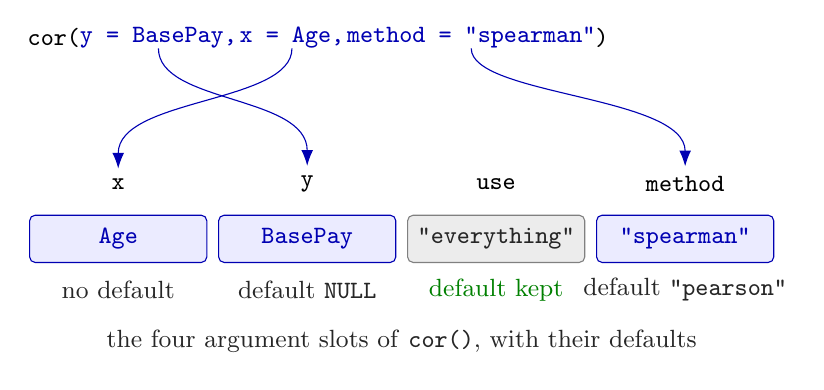
\begin{tikzpicture}[font=\small, >={Latex[length=2mm]},
  tok/.style={anchor=west, inner sep=0pt, outer sep=0pt, font=\small\ttfamily},
  slot/.style={draw, rounded corners=2pt, minimum width=2.25cm, minimum height=0.6cm, font=\small\ttfamily},
  sname/.style={font=\small\ttfamily\bfseries},
  dflt/.style={gray!30!black, font=\small}]
  % the call
  \node[tok] (c0) at (0,0) {cor(};
  \node[tok, blue!70!black] (c1) at (c0.east) {y = BasePay,};
  \node[tok] (s1) at (c1.east) {\ };
  \node[tok, blue!70!black] (c2) at (s1.east) {x = Age,};
  \node[tok] (s2) at (c2.east) {\ };
  \node[tok, blue!70!black] (c3) at (s2.east) {method = "spearman"};
  \node[tok] at (c3.east) {)};
  % the slots of cor()
  \node[gray!30!black] at (4.75,-3.85) {the four argument slots of \texttt{cor()}, with their defaults};
  \foreach \n/\x in {x/1.15, y/3.55, use/5.95, method/8.35} { \node[sname] (n\n) at (\x,-1.85) {\n}; }
  \node[slot, draw=blue!70!black, fill=blue!8, text=blue!70!black] (x) at (1.15,-2.55) {Age};
  \node[slot, draw=blue!70!black, fill=blue!8, text=blue!70!black] (y) at (3.55,-2.55) {BasePay};
  \node[slot, draw=gray, fill=gray!15, text=gray!30!black] (u) at (5.95,-2.55) {"everything"};
  \node[slot, draw=blue!70!black, fill=blue!8, text=blue!70!black] (m) at (8.35,-2.55) {"spearman"};
  \node[dflt] at (1.15,-3.2) {no default};
  \node[dflt] at (3.55,-3.2) {default \texttt{NULL}};
  \node[green!50!black] at (5.95,-3.2) {default kept};
  \node[dflt] at (8.35,-3.2) {default \texttt{"pearson"}};
  % matching arrows
  \draw[->, blue!70!black] (c1.south) .. controls +(0,-0.7) and +(0,0.9) .. (ny.north);
  \draw[->, blue!70!black] (c2.south) .. controls +(0,-0.7) and +(0,0.9) .. (nx.north);
  \draw[->, blue!70!black] (c3.south) .. controls +(0,-0.6) and +(0,0.9) .. (nmethod.north);
\end{tikzpicture}
\end{document}
